\documentclass[twocolumn]{article}
\usepackage{graphicx}
\usepackage{amsmath}
\usepackage{float}
\usepackage{amssymb} %Use of therefore symbol
\usepackage{hyperref}
\usepackage{caption}



\begin{document}
\title{Lab 2: Fourier Transforms}
\author{Alex Matheson, Austin Nhung}
%\affiliation{Department of Physics and Astronomy, University of Calgary, Calgary AB T2N 1N4 Canada}
\date{\today}
\maketitle

\section{Introduction}

\subsection{Fourier Series}
Fourier series are defined by calculating the Fourier coefficients $a_n$ and
$b_n$. These coefficients may be replaced with a complex Fourier series using
a single complex coefficient $c_n$. These coefficients are related through the
equations:
\begin{equation}
\begin{split}
a_n =& c_n + c_{-n} \\
b_n =& i(c_n - c_{-n}) \\
c_n =& \frac{1}{2}(a_n - ib_n)
\end{split}
\end{equation}
In Fourier series, $a_n$ and $b_n$ correspond to even and odd 'components' of
the function, respectively. In the case of an even function, their relations
simplify to:
\begin{equation}
\begin{split}
a_n =& c_n + c_{-n} \\
b_n =& 0 \\
c_n =& \frac{1}{2}(a_n)
\end{split}
\end{equation}

Meanwhile, odd functions simplfiy to:
\begin{equation}
\begin{split}
a_n =& 0 \\
b_n =& i(c_n - c_{-n}) \\
c_n =& \frac{-ib_n}{2}
\end{split}
\end{equation} 
 
It can be shown in both of the above series that the $a_n$ term for even
functions and $b_n$ for odd functions will be proportional to the $c_n$ terms.
The complex coefficients are alternatively defined as:
\begin{equation}
  c_n = \frac{1}{2 \pi} \int_{-\pi}^{+\pi} f(x) e^{-inx} dx
\end{equation}
It is easy to see that $c_{-n} = c_n^{\ast}$, where $c_n^{\ast}$ is the complex
conjugate of $c_n$. The relation of squares can then be expressed:
\begin{equation}
  \begin{aligned}
    \sum_{n = -\infty}^{+\infty} \left| c_n \right|^2
    &= \sum_{n = -\infty}^{+\infty} \left| \frac{1}{2} (a_n - ib_n) \right|^2 \\
    &= \frac{1}{4} \sum_{n = -\infty}^{+\infty} \left(
      \left| a_n \right| + \left| b_n \right|^2
    \right)
    &= \frac{1}{2} \sum_{n=0}^{\infty} \left(
      \left| a_n \right|^2 + \left| b_n \right|^2
    \right)
  \end{aligned}
\end{equation}
Using the definition of $b_n$, this result can be further simplified knowing
that $b_0 = i(c_0 - c_0) = 0$ to reach the final form
\begin{equation}
  \sum_{n = -\infty}^{+\infty} \left\| c_n \right\|^2
  = \left\| \frac{a_0}{2} \right\|^2 + \frac{1}{2} \sum_{n=0}^{\infty} \left(
    \left| a_n \right|^2 + \left| b_n \right|^2
  \right)
\end{equation}

Next, a square wave function was considered as defined below: 
\[ 
f(t)=
\begin{cases}
1, & |t| \leq T/4 \label{eq:square}
\\
0, & |t| > T/4
\end{cases}
\]

This function is periodic between $-T/2$ and $T/2$. The function is visualized
in figure \ref{fig:square}. As with any function, this can be restated using a
complex Fourier series. To compute the series, the coefficients $c_n$ are
determined according to equation \ref{eq:complex_coefficients}.

\begin{figure}
\centering
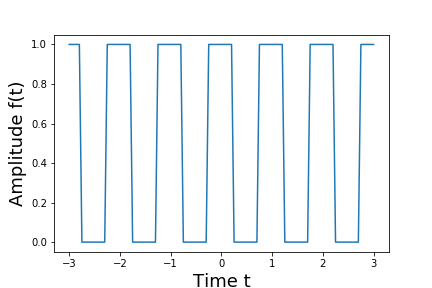
\includegraphics[width=\linewidth]{Figure1}
\caption{A square wave function. The period of the function has been set to $T=1$, periodic from $T=-1/2$ to $T=1/2$.}
\label{fig:square}
\end{figure}

\begin{equation}
c_n = \frac{1}{T} \int_{-T/2}^{T/2} f(t) \exp(-i\frac{2\pi nt}{T}) dt
\label{eq:complex_coefficients}
\end{equation}

The coefficients can be solved analytically, yielding the solution $c_n =
\frac{-i}{\pi n}$ for $n = 1, 3, 5, \ldots$. As the values of $n$ suggest, the
original function is purely odd, meaning that the function can be constructed
purely from sine terms. Due to this, all even $c_n$ terms (including $c_0$) are
$0$. The values of the different $c_n$ terms are shown in figure
\ref{fig:Figure2}. The values in this plot show that the odd $n$ terms follow a
hyperbolic sinusoid path. The complete series may be written as:
\[
f(t) = \sum_{n= -\infty}^{\infty} -\frac{i}{\pi n} \exp(-i \frac{2\pi nt}{T})
\]

\begin{figure}
\centering
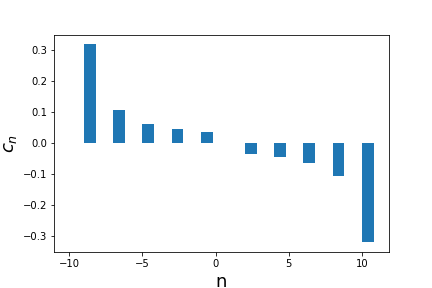
\includegraphics[width=\linewidth]{Figure2}
\caption{Values of each term $c_n$ in the complex fourier series.}
\label{fig:Figure2}
\end{figure}


\subsection{FFT}
Four simple analog signals were used to analyze the behaviour and consequences
of sampling a signal and using the discrete Fourier transform. The signals used
were:
\begin{equation}
  \begin{aligned}
    f_1(t)  &= \sin(2 \pi \times 100 t) + \frac{1}{2} \sin(2 \pi \times 200 t) \\
    f_2(t) &= \sin(2 \pi \times 100.5 t) + \frac{1}{2} \sin(2 \pi \times 200 t) \\
    f_3(t) &= \left( 2 + \sin(2 \pi \times 8 t) \right) \times \sin(2 \pi \times 100 t) \\
    f_4(t) &= \sin \left( 2 \pi \times 100 \left( 1 + \frac{1}{10} \sin(2 \pi \times 8 t) \right) t \right)
  \end{aligned}
  \label{fft_eqs}
\end{equation}

These signals were sampled at a rate of $1024$ samples per second for one second
each. They were then transformed into the frequency domain using the fast
Fourier transform (FFT). The amplitudes and power spectra are shown in figure

\ref{fig:fft_exs}.
\begin{figure*}
  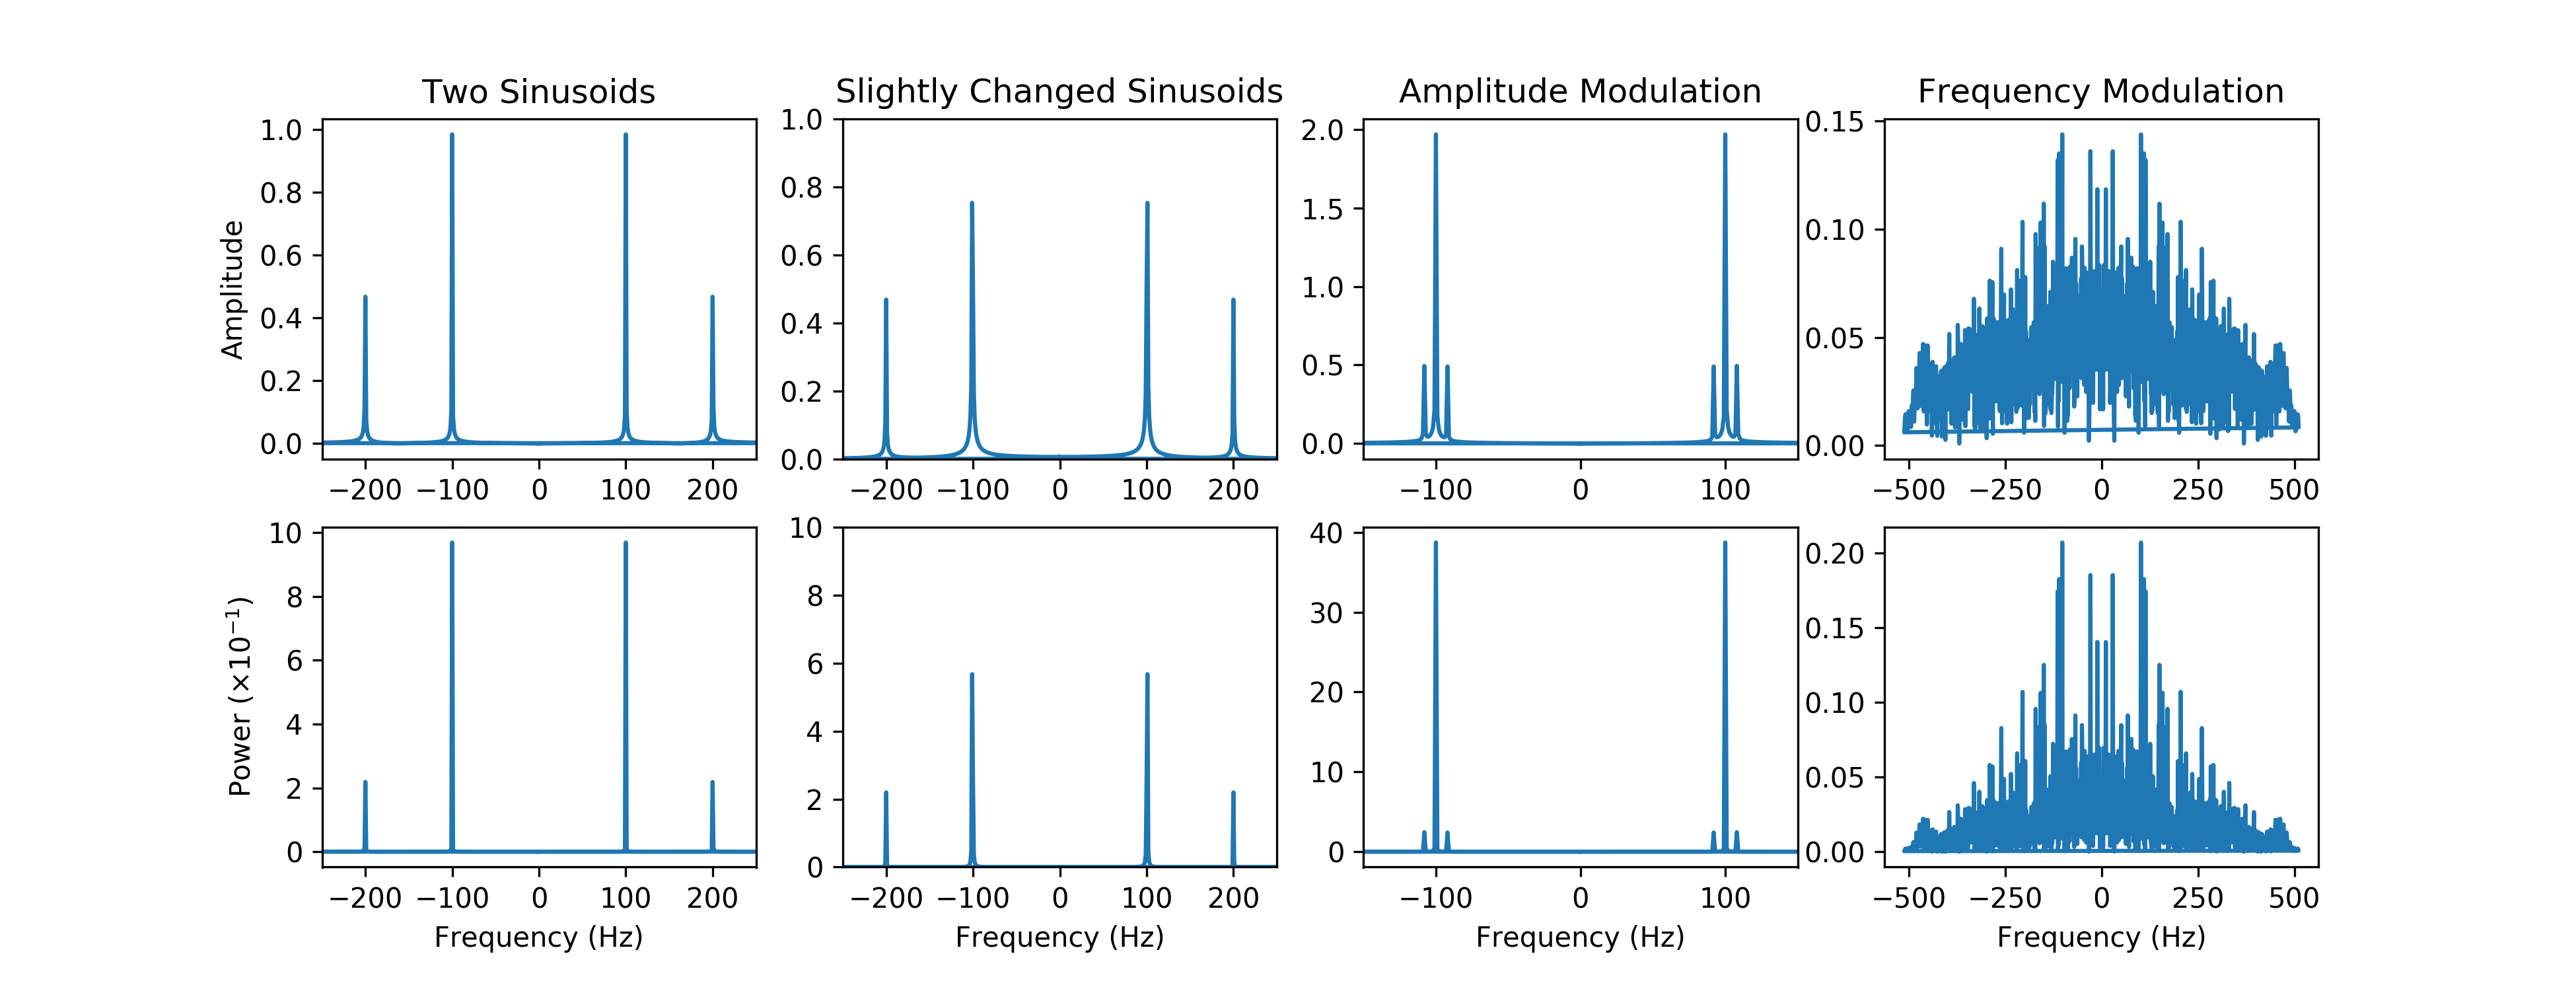
\includegraphics[width=\pagewidth]{fft_examples.png}
  \caption{
    The amplitude (top row) and corresponding power (bottom row) spectra of the
    signals described in \ref{fft_eqs} in the same order from left to right.
  }
  \label{fig:fft_exs}
\end{figure*}

The first signal is simply the sum of two sines at frequencies $100$Hz and
$200$Hz with amplitudes $1$ and $0.5$, respectively. This is evident on the
two leftmost panels in figure \ref{fig:fft_exs}. The second signal is only
slightly different from the first, yet the amplitude and width of the peak at
$100$Hz is noticably different. This is because the number of samples limits the
number of bins that will be calculated and the sampling frequency limits the
highest frequency. Since the sampling rate is $1024$Hz and there are $1024$
samples, each frequency bin is $2$Hz. $100$Hz was easily resolved since it is a
multiple of $2$, but this is also the reason why $100.5$Hz was not.

The other signals are examples of amplitude and frequency modulation. The
amplitude modulated signal involves multiplying sines together, which can be
expressed as:
\begin{equation}
  \sin(\alpha) \times \sin(\beta) = \frac{1}{2} \left(
    \cos(\alpha - \beta) - \cos(\alpha + \beta)
  \right)
\end{equation}
This is the resulting signal in the third column of figure \ref{fig:fft_exs}
where the peaks occur at $100$Hz as well as $100 \plusminus 8$Hz. Frequency
modulation can be thought of as varying the frequency of the signal over time.
This is the reason that its Fourier transform is spread across the entire range
of frequencies.


\subsection{Noise}
\subsubsection{Autocorrelation and PSD}
The autocorrelation function was examined in a previous lab. It turns out that the auto-correlation function may be applied to random signals (i.e. noise) as well. For white noise created from a uniform distribution of frequencies, the autocorrelation function is expected to be a delta function. Consider an ideal random number generator separate from the realities of computing. By definition, a number correlates with itself completely, forming a spike at $k=0$. For ideal noise, there is no relation between the first number generated, and any subsequent number generated. This means that subsequent values should yield $k=0$. Taken together, this is a description of $\delta(k)$.

The power spectral density function is connected to the auto-correlation function by the following formula:

\[ S(\omega) = \sum_{-\infty}^{\infty} AC(k)e^{-j\omega k} \]

Using this, the PSD of white noise may be calculated:

\[ S(\omega) =  \sum_{i=-\infty}^{\infty} \delta (k) e^{-j\omega k}\\
S(\omega) = \delta(k=0) e^{-j\omega * 0} \\
S(\omega) = 1
\] 

The above mathematical relations were tested 

% FIGURE OUT THE PROBLEM WITH THE AUTOCORRELATION FUNCTION

\subsection{Spectral Subtraction}
The spectral subtraction method involved Fourier transforming a signal, and then setting frequency bin values to zero if they were below a certain threshold. A signal was created using the formula $ x(t) = \sin (2\pi f_0t) + 0.5\sin (2\pi (2f_0)t)$ using $f_0=440$ Hz sampled at $22.2\mu s$, for $512$ intervals. Figure\ref{fig:spectral_filter}a shows this signal. The power spectrum of the signal was found using numpy's FFT package. Figure \ref{fig:spectral_filter}b shows this corresponding power spectrum. Two clear peaks were visible at $0.00976$ and $0.01953$. This matches almost exactly the expected values of $0.9768$ and $0.19536$ obtained by multiplying the frequency by the sampling period.

To investigate the impact of noise on the signal, random noise on the order $\pm 0.5$ was added to the signal. Figures \ref{fig:spectral_filter}c and \ref{fig:spectral_filter}d show the noisy power spectrum. The noise in this power spectrum was almost imperceptible compared to the signal in the neighborhood of the expected peaks. By outputting the power data, it was seen that the noise was on the order of $10^{-1}$. Some noise was slightly beyond one order of magnitude above or below this, indicating that the noise was not 'ideal' white noise.

Next, the threshold at which the magnitude of the noise cause the underlying signal to be totally obscured was determined. This was done by steadily increasing the noise magnitude until the signal peaks were on the order of the peaks from noise. Figure \ref{fig:spectral_filter}e and \ref{fig:spectral_filter}f show the corresponding signal and power spectrum.


\begin{figure*}[t]
	\centering
	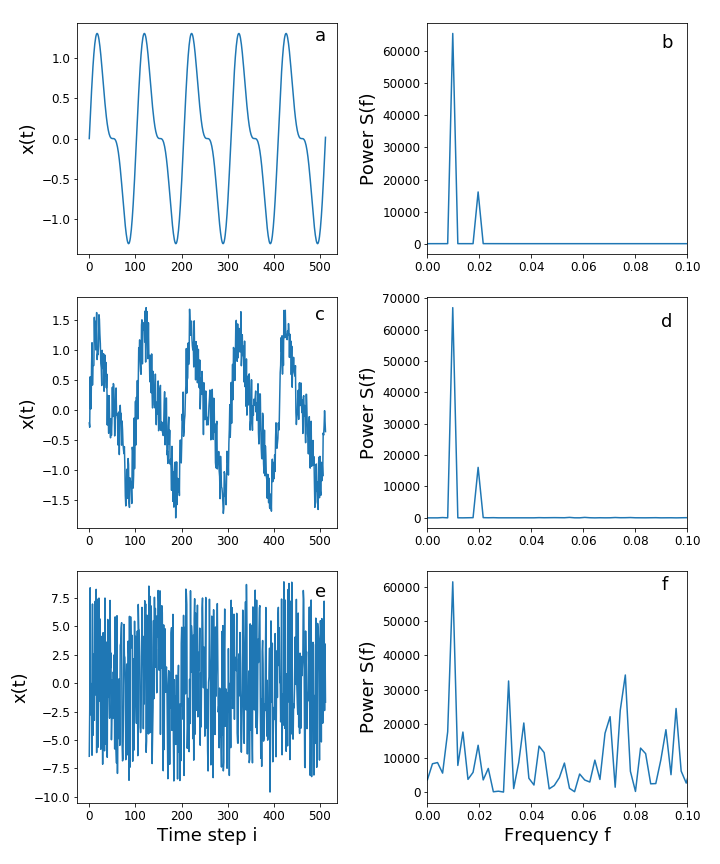
\includegraphics[height=\paperwidth]{spectral_filter}
	\caption{Effects of uniformly distributed (in time space) noise on a signal. Subplot \textbf{a} shows the original input signal, subplot \textbf{c} a signal with noise of $\pm0.5$ from the original signal, and subplot \textbf{e} the signal with $\pm10$ noise. The subplots immediately to the right are the corresponding frequency power spectra.}
	\label{fig:spectral_filter}
\end{figure*}

\subsubsection{Signals with Trends}
In this section, a periodic signal was laid over a linear trend to produce a new function. The original periodic function was $x_i = 2\sin(\pi f_0 i) + \cos( \pi f_1 i)$ while the trend function was $g(i) = 1 + 0.025i$ (constants of $f_0 = 9/512$ and $f_1=4/512$ were used). When added together, the two functions produced a new function, visualized in figure \ref{fig:trend}.
Next, the signal was made noisy using uniform noise of $\pm6$ added to the function. Figure \ref{noise_trend} shows the result.

\begin{figure}
\centering
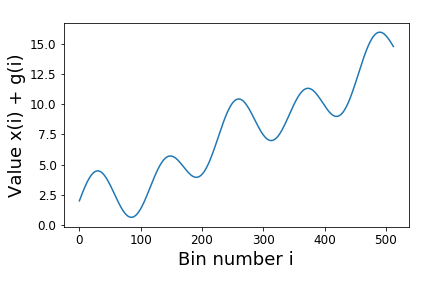
\includegraphics[width=\linewidth]{trend}
\caption{Function obtained by adding together a periodic and a linear function.}
\label{fig:trend}
\end{figure}

\begin{figure}
\centering
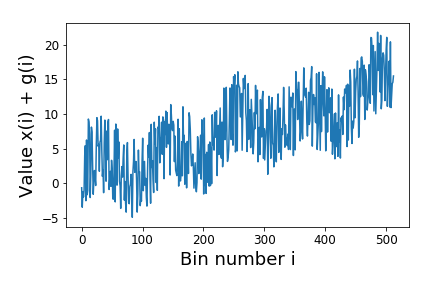
\includegraphics[width=\linewidth]{noise_trend}
\caption{Function from figure \ref{fig:trend} with uniform noise applied.}
\label{fig:noise_trend}
\end{figure}

As earlier in this lab, the FFT was used to examine the data for the underlying periodicity. Figure \ref{fig:trend_fft} showed the resulting power spectrum. The data was confined to a single, massive spike at $f=0$. For a noisy signal, the noise would be expected to manifest as a uniform addition across the power spectrum. This would still allow the original frequencies to be recovered. The lack of any distinct periodic peaks (the $f=0$ peak corresponds to non-periodic components) suggests that the linear component has erased the ability to check periodicity in the power spectrum. 

\begin{figure}
\centering
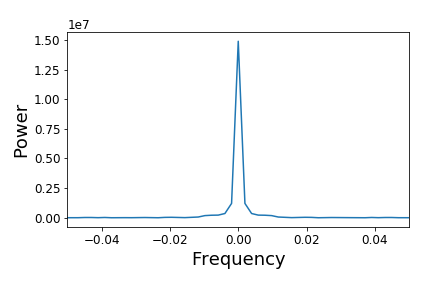
\includegraphics[width=\linewidth]{trend_fft}
\caption{FFT of the noisy function in figure \ref{fig:noise_trend}. The result was focused on the region near $f=0$ to ensure that there were not peaks close to $f=0$. Regions outside this window continued at an amplitude of approximately zero. Note that the amplitude axis is scaled by a factor of $10^{7}$.}
\label{fig:trend_fft}
\end{figure}

While it has been shown that the periodicity of the data are obscured, it might have still been possible to remove the noise across all frequencies, and attempt to recover the original, noiseless function. To attempt this, all frequencies with a magnitude of less than $180$ were removed. Figure \ref{fig:Reconstruction} shows the result. Clearly this method has not been successful. 

\begin{figure}
\centering
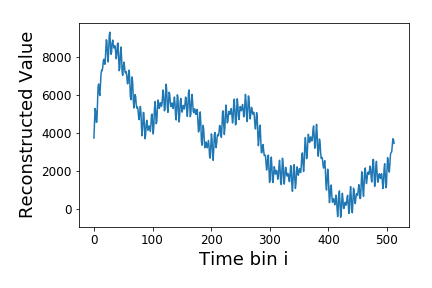
\includegraphics[width=\linewidth]{Reconstruction}
\caption{Reconstruction of the signal in figure \ref{fig:trend} using an inverse FFT. Note that the trend $g(i)$ does not appear as expected in the reconstruction. This result was one of many: each separate run of the program produced a different reconstruction based on the different random noise changes.}
\label{fig:Reconstruction}
\end{figure}

Next, a different method of uncovering the original $x(i)$ function was attempted. First, the $g(i)$ term was removed from $x(i)$. This new modified $x(i)$ was then Fourier transformed. The noise was again removed from the signal using only frequency magnitudes greater that $180$. It was found that using the suggested filtering value of 9 from the lab instructions did not yield the correct results. Using the filtered frequency spectrum, the inverse Fourier transform, that is the noiseless $x(i) - g(i)$ was obtained. Finally, the trend $g(i)$ was added back to the signal. Originally, this yielded a massive sinusoid without upward trend. To fix this, after the frequency spectrum was returned to the time domain, the result was re-normalized to the maximum of the original trend-less $x(i)$. This was cheating somewhat, as in real experiments, the maximum of the original function might not be known. Once the signal was re-normalized and had $g(i)$ added back in, the signal behaved more similarly to what was expected. Figure \ref{reconstruction_fixed} shows the final result.

\begin{figure}
\centering
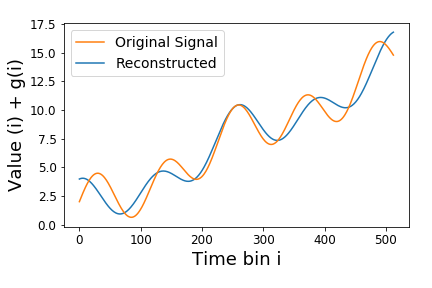
\includegraphics[width=\linewidth]{reconstruction_fixed}
\caption{Reconstruction of the original signal from figure \ref{fig:trend}. Note the aparent scale difference between the two lines.}
\label{fig:reconstruction_fixed}
\end{figure}

\subsubsection{Autocorrelation and Power Spectra}
The autocorrelation function and the power spectrum of signals are related. This may be demonstrated analytically with relative ease. Essential to these derivations is the Fourier shift theorem. The theorem provides a quick way to simply a Fourier transform when the function in question contains a shift in the coordinate being transformed. The theorem is derived below:
\begin{equation}
\begin{split}
\mathcal{F} \{f(t - a)\} = & \int_{-\infty}^{\infty} f(t-a) e^{2\pi i\omega t} dt \\
= & \int_{-\infty}^{\infty} f(t-a) e^{2\pi i\omega t} e^{2\pi i\omega a} e^{-2\pi i\omega a} dt \\
= & e^{2\pi i\omega a} \int_{-\infty}^{\infty} f(t-a) e^{2\pi i\omega t}  e^{-2\pi i\omega a} dt \\
= & e^{2\pi i\omega a} \int_{-\infty}^{\infty} f(t-a) e^{2\pi i\omega (t - a)} dt \\
= & e^{2\pi i\omega a} \int_{-\infty}^{\infty} f(t') e^{2\pi i\omega t'} dt' \\
= & e^{2\pi i\omega a} \mathcal{F} \{f(t)\}
\end{split}
\end{equation}

First, a proof will be shown for $C(\omega) = \sqrt{2\pi} Y^*(\omega)X^*(\omega)$:

\begin{equation}
\begin{split}
c(\tau) = & \int_{-\infty}^{\infty} y^*(t - \tau) x(t) dt\\
\mathcal{F} \{c(\tau)\} = & \mathcal{F} \{\int_{-\infty}^{\infty} y^*(t - \tau) x(t) dt\} \\
C(\omega) = & \int_{-\infty}^{\infty} \int_{-\infty}^{\infty} y^*(t - \tau) x(t) e^{2\pi i \omega \tau} dt d\tau \\
= & \int_{-\infty}^{\infty} \int_{-\infty}^{\infty} y^*(-\tau) x(t) e^{2\pi i \omega t} e^{2\pi i \omega \tau} dt d\tau \\
= & \int_{-\infty}^{\infty}y^*(\tau) e^{2\pi i \omega (-\tau)}  d\tau \int_{-\infty}^{\infty}  x(t)  e^{2\pi i \omega t} dt \\
= &\sqrt{2\pi} Y^*(\omega)X(\omega)
\end{split}
\end{equation}

Related to the correlation function is the autocorrelation function. The autocorrelation function may be defined as a convolution of a function with itself. From this term's Fourier material, it has been stated that a convolution in one space is a product in the corresponding Fourier space. From this, the relation between the autocorrelation and the power spectrum of a signal have been linked. This may be proved, as shown below:

\begin{equation}
\begin{split}
AC(\tau) = & \int_{-\infty}^{\infty} y^*(t) y(t + \tau) dt\\
\mathcal{F} \{AC(\tau)\} = & \mathcal{F} \{\int_{-\infty}^{\infty} y^*(t - \tau) y(t) dt\} \\
AC(\omega) = & \int_{-\infty}^{\infty} \int_{-\infty}^{\infty} y^*(t - \tau) y(t) e^{2\pi i \omega \tau} dt d\tau \\
= & \int_{-\infty}^{\infty} \int_{-\infty}^{\infty} y^*(-\tau) y(t) e^{2\pi i \omega t} e^{2\pi i \omega \tau} dt d\tau \\
= & \int_{-\infty}^{\infty}y^*(\tau) e^{2\pi i \omega (-\tau)}  d\tau \int_{-\infty}^{\infty}  y(t)  e^{2\pi i \omega t} dt \\
= &\sqrt{2\pi} Y^*(\omega)Y(\omega) \\
= & \sqrt{2\pi} |Y(\omega)|^2
\end{split}
\end{equation}

The auto-correlation function of white noise was explored earlier in this assignment. The findings of that computation may be verified analytically. Given that white noise should exist equally at all, infinite frequencies in the frequency domain, the autocorrelation may be determined by reverse Fourier transform. To begin, an assumption is made that the power of all frequencies is $S(f) = k$.
\begin{equation}
\begin{split}
S(f) =& k \\
AC(\tau) =& \mathcal{F}^{-1} \{ S(f) \} \\
AC(\tau) =& \sqrt{2\pi} \int_{-\infty}^{\infty} k e^{-2\pi i f \tau} df \\
AC(\tau) =& \sqrt{2\pi}k \int_{-\infty}^{\infty} e^{- i \omega \tau} \frac{d\omega}{2\pi} \\
AC(\tau) =& \frac{k}{\sqrt{2\pi}} \int_{-\infty}^{\infty} e^{- i \omega \tau} d\omega \\
AC(\tau) =& \frac{k}{\sqrt{2\pi}} \delta(\tau) \\
\end{split}
\end{equation}


\section{Applications}

\subsection{The Lorenz System}
The Lorenz system is a description of physical systems where a large number of variables are interrelated through differential equations. For this example, a system with three variables and three parameters will be considered. Equations \ref{difs} shows the system of equations in question.
\begin{equation} \label{difs}
\begin{split}
\frac{\partial x}{\partial t} =& \sigma (y - x) \\
\frac{\partial y}{\partial t} =& rx - y - xz \\
\frac{\partial y}{\partial t} =& xy - bz \\
\end{split}
\end{equation}

The equation will reach an equilibrium in the case where all the partial derivatives are zero. The $x$, $y$, and $z$ equilibrium values may be found analytically:
\begin{equation} \label{equilibrium}
\begin{split}
0 = \sigma (y - x) \quad \to  & \quad x = y\\
0 = xy - bz \quad \to & \quad y = \sqrt{(bz)}\\
0 = rx - y - xz \quad \to & \quad z = r-1\\
\therefore x = y =& \sqrt{b(r-1)}
\end{split}
\end{equation}
This is only true if $x = y \neq 0$. Otherwise, the other equilibrium state is
when all positions are at zero: $x = y = z = 0$.

Numerical solutions to the Lorenz equations were calculated using the
fourth-order Runge-Kutta scheme (RK4). In the first batch of simulations run,
different initial conditions were used while keeping the other variables
constant, with $\sigma = 10, b = 8/3, r = 28$. The phase spaces from these
simulations are shown in figure \ref{fig:sims_init}.

\begin{figure}
  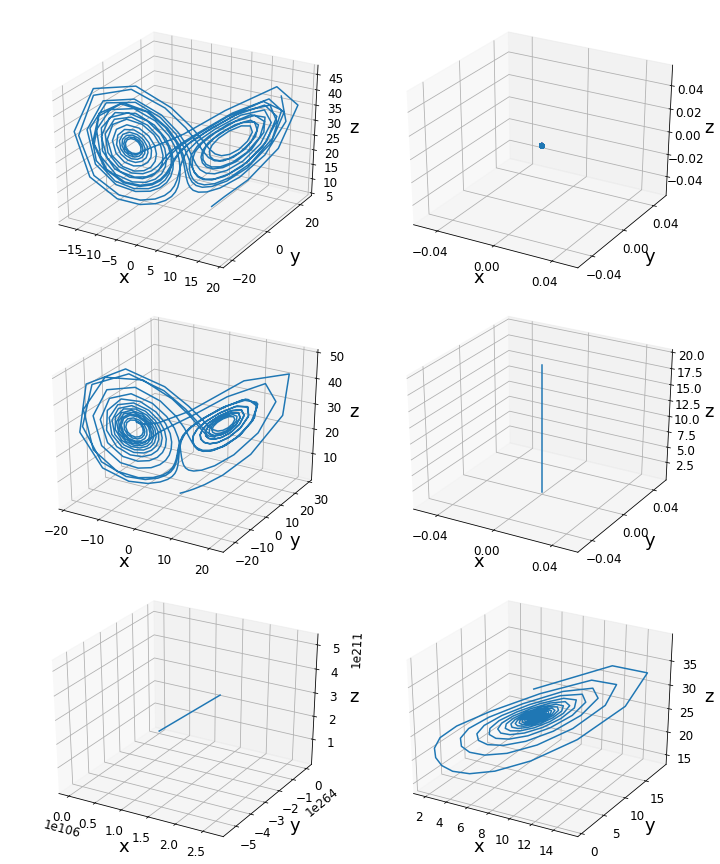
\includegraphics[width=\linewidth]{sims1.png}
  \caption{
    Simulations of the Lorenz system with varying initial conditions. The
    variables that remained constant are $\sigma=10, b=8/3, r=28$. Starting from
    the initial conditions are, from the top left, $(x_0, y_0, z_0) = \left\{
    (5, 5, 5), (0, 0, 0), (0.1, 0.1, 0.1), (0, 0, 20), (100, 100, 100), (8.5,
    8.5, 27) \right\}$.
  }
  \label{fig:sims_init}
\end{figure}

The top left panel begins with the initial condition $(x_0, y_0, z_0) = (5, 5,
5)$, and it is evident that one of the reasons that Lorenz may have used the
term ``butterfly'' to describe the evolution of this system because the solution
maps out two wings at an angle like a butterfly's. From the simulations, there
are three general ways the simulation can end up: orbiting in the butterfly
wings, come to a halt at the equilibrium points, or move completely out of the
any periodic system.

\begin{figure}
  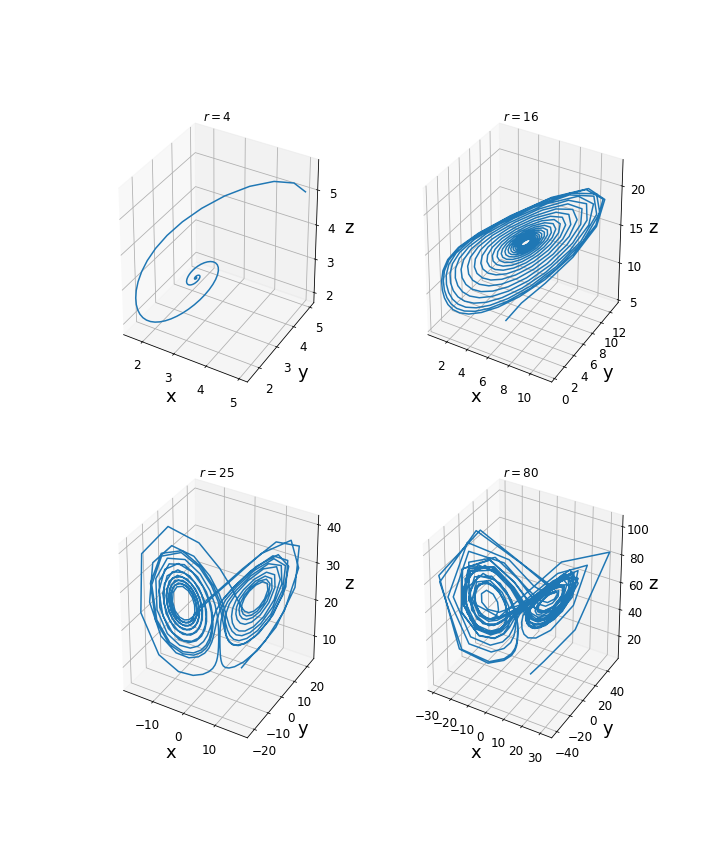
\includegraphics[width=\linewidth]{sims2.png}
  \caption{
    Simulations of the Lorenz system while varying the variable $r$. All other
    variables remain constant at $\sigma=10, b=8/3$ and initial condition $(x_0,
    y_0, z_0) = (5, 5, 5)$.
  }
  \label{fig:sims_vary_r}
\end{figure}

The second batch of simulations vary the value of $r$ and starting all of them
with the initial condition $(x_0, y_0, z_0) = (5, 5, 5)$, shown in figure
\ref{fig:sims_vary_r}. When the value is $0 < r < 24.74$, the system evolves as
a spiral, spiraling outwards faster as the value of $r$ decreases. In the other
regime, when $27.74 < r < 100$, system remains in orbit about the two butterfly
wings, with the steps increasing in size as the value of $r$ increases.

\begin{figure}
  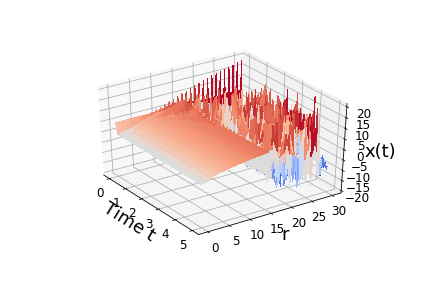
\includegraphics[width=\linewidth]{bifurcation.png}
  \caption{
    The bifurcation diagram of the Lorenz system obtained by gradually changing
    the value of $r$ from $0$ to $30$.
  }
  \label{fig:bifurcation}
\end{figure}

To further investigate the effect of $r$ on the system, the value was gradually
increased from $0$ to $30$ to create a bifurcation diagram of the Lorenz system,
shown in figure \ref{fig:bifurcation}. Once the value of $r$ was raised to the
value $27.74$, the system began to show pitchfork bifurcation, where the number
of fixed points transitions from one to three.

\subsubsection{The Fourier Analysis}

\subsection{ODEs and the Fourier Transform}
The Fourier transform can be use to reduce the dimensionality of a differential equation. In essence, if the fourier transform is used, a PDE with two different differentials may be reduced to an ODE or and ODE to a polynomial equation. The original solution may then be recovered by reverse transforming the result. Below are a few examples of simplifying differential equations through Fourier transform:

\begin{equation}
\begin{split}
\mathcal{F} \{ m\ddot{x} + D\dot{x} + \kappa x &= n(t) \} \\
-\omega^2 \hat{x} +i\omega \hat{x} + \kappa\hat{x} &= \hat{n}(\omega)
\end{split}
\end{equation}

\begin{equation}
\begin{split}
\mathcal{F} \{ih \frac{\partial \psi}{\partial t} + \frac{h^2}{2m} \frac{\partial^2 \psi}{\partial x^2} &= 0 \} \\
-\omega h \hat{\psi} - \frac{ih^2}{2m} \frac{\partial^2 \hat{\psi}}{\partial x^2} = 0
\end{split}
\end{equation}

\begin{equation}
\begin{split}
\mathcal{F} \{ \frac{\partial^2 T}{\partial x^2} + \frac{\partial^2 T}{\partial z^2} &= \delta (x) \delta (z - a) \}\\
-k^2 \hat{T} + \frac{\partial^2 \hat{T}}{\partial z^2} &= e^{-2\pi ik x} \delta (z - a)
\end{split}
\end{equation}

\subsubsection{Heat Equation}
A common differential equation that is difficult to solve with non-complex analysis was the heat equation. The heat equation was defined as:
\begin{equation}
\begin{split}
\frac{\partial^2 T}{\partial x^2} &= -q(x)\\
q(x) =& \frac{\exp(-(x-x_0)^2/(2\sigma^2))}{\sqrt{2\pi\sigma^2}}
\end{split}
\end{equation}

This equation may be re-written using Fourier analysis. Two aids were used in this analysis: an integral table result for a zero-mean gaussian transform \cite{gauss_trans}, and the Fourier shift theorem to take care of the $x_0$ shift. Equations \ref{eq:gauss_transform} show this process.

\begin{equation}
\begin{split}
&\mathcal{F}\{ \frac{\partial^2 T}{\partial x^2} \} = \mathcal{F} \{ -q(x) \} \\
&-k^2 \hat{T} = -\hat{q}(x) \\
%&\\
%\hat{q}(x) =& \mathcal{F} \{ \frac{\exp(-(x-x_0)^2/(2\sigma^2))}{\sqrt{2\pi\sigma^2}} \} \\
%\hat{q}(x) =& e^{-2\pi ikx_0} \times \mathcal{F} \{ \frac{\exp(-(x^2/(2\sigma^2))}{\sqrt{2\pi\sigma^2}} \} \\
%\hat{q}(x) =& \exp\bigg( \frac{-\sigma^2 k^2}{2} - 2\pi ikx_0 \bigg) \\
%\hat{T} =& \frac{1}{k^2} \exp\bigg( \frac{-\sigma^2 k^2}{2} - 2\pi ikx_0 \bigg)
%
%\hat{q}(x) =& \frac{1}{\sqrt{2\pi\sigma^2}} \int_{-\infty}^{\infty} e^{2\pi ikx} e^{-(x-x_0)^2/\sqrt{2\sigma^2}} dx \\
%\hat{q}(x) =& \frac{1}{\sqrt{2\pi\sigma^2}} \int_{-\infty}^{\infty} \cos(2\pi kx) e^{-(x-x_0)^2/\sqrt{2\sigma^2}} dx \\
%\hat{q}(x) =& \frac{1}{\sqrt{2\pi\sigma^2}} e^{-2\pi ikx_0} \int_{-\infty}^{\infty} \cos(2\pi kx) e^{-x^2/\sqrt{2\sigma^2}} dx \\
%\hat{q}(x) =& \frac{1}{\sqrt{2\sigma^2}} e^{-2\pi ikx_0} \sqrt{\pi\sqrt{2\pi\sigma^2}} e^{-\pi^2 k^2 \sqrt{2\sigma^2}} \\
%\hat{T} &= \frac{e^{-\pi^2 k^2\sqrt{2\sigma^2} - 2\pi ikx_0/(2\sigma)^2}}{\sqrt{2k\pi\sigma^2}}
\end{split}
\label{eq:gauss_transform}
\end{equation}

In order to numerically solve the heat equation, the function $q(x)$ should be Fourier transformed to obtain $\hat{q}(k)$. This term may then be divided by $k^2$ and reverse transformed to obtain the original $T(x)$. This yields a problem in the case where $k=0$. Since python interprets a division by zero by returning 'nan'', replacing this 'nan' with some DC term will allow the inverse transform to perform correctly. Figure \ref{fig:temp} shows the result of performing this method. Since the 'DC' term for $k=0$ has been replaced, this is not the exact answer, and instead is shifted by the non-existent DC term. It was therefore possible to shift this data so that all points had a non-negative temperature by shifting by the global minimum value. 

\begin{figure}
\centering
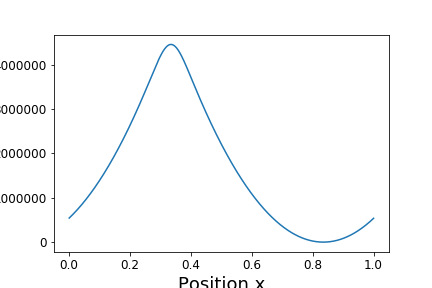
\includegraphics[width=\linewidth]{temp}
\caption{Temperature of a length $1$ rod corresponding to equation \ref{?}. The temperature may be off by a constant shift due to the deletion of the DC component in the frequency space.}
\label{fig:temp}
\end{figure}

The limits of Fourier transform solutions were considered using the function $q(x) = 0$. For this case, the familar solution of $T(x) = Ax + B$ was obtained using analytical methods. For this particular case, the Fourier method of solutions breaks down. If we were to Fourier transform $q(x)$, the result would be $q(k)=0$. This in turn would lead to an overall solution $T(x) = 0$. This is a valid solution for the analysis above in the case $A=B=0$, however it is only one possible solution out of many.


\section{Conclusion}



\begin{thebibliography}{00}
	\bibitem{ouyed}
	Ouyed and Dobler, PHYS 581 course notes, Department of Physics and Astrophysics, University of Calgary (2016).
	\bibitem{NR}
	W. Press et al., \emph{Numerical Recipes} (Cambridge University Press, 2010) 2nd. Ed.
	\bibitem{Code}
	C. Hass and J. Burniston, MCMC Hill Climbing. Jupyter notebook, 2018.
	\bibitem{gauss_trans}
	K. Derpanis, Fourier Transform of the Gaussian, 2005, accessed at \url{http://www.cse.yorku.ca/~kosta/CompVis_Notes/fourier_transform_Gaussian.pdf}.
\end{thebibliography}

\section{Appendix}
For access to the source codes used in this project, please visit \url{https://github.com/Tsintsuntsini/PHYS_581} for a list of files and times of most recent update.
	
\end{document}